\documentclass[openany]{book}

% Dimensione pagina e margini
% 'a4paper' è lo standard EU/UK, altrimenti metti altro
\usepackage[a4paper,top=2cm,bottom=2cm,left=3cm,right=3cm,marginparwidth=1.75cm]{geometry}

% Lista package utili generici
\usepackage{amssymb}
\usepackage{amsmath}
\usepackage{graphicx}
\usepackage[colorlinks=true, allcolors=black]{hyperref}
\usepackage[italian]{babel}
\usepackage{color,soul}
\usepackage{cancel}
\usepackage{wrapfig}
\usepackage{caption}
\usepackage{forest}
\usepackage{tikz-qtree}
\usepackage[utf8]{inputenc}

% Box per definizioni, c, python e bash
\usepackage{Style/code_boxes}

% Box per codice simile a math_boxes
\usepackage{Style/new_code_boxes}

% Box per matemarica
\usepackage{Style/math_boxes}

% Per bibliografia
\usepackage{csquotes}
\usepackage[backend=biber, style=numeric, sorting=none]{biblatex}
\addbibresource{ref.bib}

% Titolo indice più grande
\renewcommand{\contentsname}{\huge{Indice}}

% Le pagine vuote non hanno numero
\makeatletter
\def\cleardoublepage{\clearpage\if@twoside \ifodd\c@page\else
\hbox{}
\thispagestyle{empty}
\newpage
\if@twocolumn\hbox{}\newpage\fi\fi\fi}
\makeatother


%------------------------------------------------
%	Inizio documento
%------------------------------------------------
\begin{document}

%------------------------------------------------
%	Copertina
%------------------------------------------------
\begin{titlepage}
  \begin{center}
    
\includegraphics[width=15cm]{Images/Unimore.jpg} \\
    \vspace{1cm}
    {\LARGE{ UNIVERSITÀ DEGLI STUDI DI MODENA \\E REGGIO EMILIA \\}}
    {\large{ Dipartimento di Ingegneria "Enzo Ferrari" \\}}
    {\large{ Corso di Laurea Triennale in Ingegneria Informatica (L-08) \\}}
    \vspace{3cm}
    {\Large { \textbf{Traffic Shaping in Userspace: Fattibilità e Limiti} }}\\
    \vspace{3cm}
  \end{center}
  \begin{minipage}[t]{0.47\textwidth}
    {\large{\bf Tutor:}\\} 
    {\large Prof. Riccardo Lancellotti}
  \end{minipage}\hfill\begin{minipage}[t]{0.47\textwidth}\raggedleft
  {\large{\bf Candidato:}\\}
  {\large Leonardo Donati}\\
  {\large Matricola 191271}
  \end{minipage}
  \vfill
  \hrulefill\\
  \centering{\large{\bf ANNO ACCADEMICO 2025/2026 }}
 \end{titlepage}

%------------------------------------------------
%	Indice
%------------------------------------------------
\newpage
\centering
\tableofcontents

%------------------------------------------------
%	Inizio appunti
%------------------------------------------------
\raggedright
\chapter{Introduzione}
Il traffic shaping è una tecnica ampiamente utilizzata nelle reti informatiche per controllare la larghezza di banda disponibile a utenti, servizi o flussi di traffico specifici. 
In ambienti Linux, è possibile tramite il comando \texttt{tc}, che agisce direttamente all'interno del kernel utilizzando diverse queueing discipline. \\
\vspace*{0.01\textheight}
Questo approccio presenta un limite in ambienti containerizzati: non disponendo di un kernel proprio, un container usa le funzionalità di rete messe a disposizione dal kernel dell'host.
L'assenza dei moduli necessari al comando \texttt{tc} può quindi creare problemi con portabilità e riproducibilità di uno scenario di rete in diversi sistemi. \\
\vspace*{0.01\textheight}
L'obiettivo di questa tesi è verificare la fattibilità di un approccio alternativo, che sposti la logica di traffic shaping dal kernel allo spazio utente con il framework Netfilter e le code NFQUEUE. \\
\vspace*{0.01\textheight}
La tesi è strutturata come segue: il capitolo 2 introduce il traffic shaping in ambienti Linux, con le discipline di accodamento TBF e HTB.
Il capitolo 3 mostra il funzionamento di Kathará, il programma usato per le simulazioni degli scenari di rete e i suoi limiti. Il capitolo 4 spiega l'approccio di traffic shaping in userspace e del framework Nelfilter. 
Il capitolo 5 ne dimostra la fattibilità tramite il programma Damper, evidenziato i suoi limiti strutturali. 
Infine, il capitolo 6 descrive in modo dettagliato il fork Donper, che permette di gestire classi e condivisione di banda in modo simile, ma non uguale, alla qdisc spiegate nel capitolo 1.

\chapter{Traffic Shaping}

%  Definizione traffic shaping generale
\section{Definizione}
\begin{defn}[Traffic Shaping]
  Il traffic shaping è una tecnica di gestione della larghezza di banda utilizzata nelle reti informatiche,
  che ritarda alcuni o tutti i datagrammi IP per adeguarli al profilo di traffico desiderato.
  Consente di migliorare le prestazioni della rete controllando in il traffico in entrata e in uscita o di simulare condizioni di reti reali.
\end{defn}
A differenza di tecniche basate sullo scarto di datagrammi IP in eccesso, il traffic shaping ne ritarda l'invio, trattendoli in una coda. \\
Esistono alcuni scenari tipici in cui è applicato:
\begin{itemize}
  \item \textbf{Limitazione} della banda per utenti e servizi in una rete;
  \item \textbf{Garanzia} di banda minima per determinati flussi;
  \item \textbf{Prioritizzazione} del traffico;
  \item \textbf{Minimizzazione} della latenza;
\end{itemize}

% Traffci shaping su Linux
\section{Traffic Shaping in Ambienti Linux}
In ambienti Linux il traffic shaping può essere effettuato con il comando \texttt{tc} (traffic control) \cite{tc}, disponibile nella suite di comandi \texttt{iproute2} \cite{iproute2}.\\
Nella pagina ufficiale del manuale di \cite{tc}, viene evidenziato come l'elaborazione del traffico è gestita tramite tre tipi di oggetti: \textbf{qdisc}, \textbf{classi} e \textbf{filtri}.

\subsection{Queueing Discipline (qdisc)}
\begin{defn}[qdisc]
  qdisc è l'abbreviazione di queueing discipline: rappresenta il meccanismo con cui il kernel gestisce l'invio dei pacchetti su un'interfaccia,
  accodandoli secondo una politica configurabile \cite{tc}.
\end{defn}
Alcune qdisc possono essere \textbf{classful}, quindi contenere classi con con a loro volta una propria qdisc, creando di fatto una gerarchia.
Il kernel può decidere di inviare un pacchetto di una classe invece che un'altra, per dare priorità a determinati tipi di traffico cercando di estrarre pacchetti prima da certe classi. \\
\vspace*{0.01\textheight}
Eventualmente, le qdisc possono essere pure \textbf{classles}, potendo solo riordinare, ritardare o scartare pacchetti.

\subsection{Token Bucket Filter (TBF)}
\begin{defn}[Token Bucket Filter]
  Disciplina di accodamento \textbf{classles} disponibile per il controllo del traffico nel comando \texttt{tc}.
  Funziona puramente da shaper e non si occupa mai dello scheduling del traffico. \cite{tc-tbf}
\end{defn}
TBF è molto leggero e non appesantisce la rete né il processore. Il suo unico limite è che può lavorare su una interfaccia usando una sola coda.

\subsubsection{Algoritmo}
L'implementazione consiste in un buffer (\textbf{bucket}) che viene costantemente riempito di gettoni (\textbf{tokens}), a una velocità specifica \textbf{rate}.
Il bucket ha un capienza (\textbf{burst}), che indica quanti gettoni può contenre al massimo. Un token equivale a circa un byte. \\ 
\vspace*{0.01\textheight}
Quando un pacchetto deve essere inviato, i gettoni necessari per inviarlo vengono rimossi dal bucket.
Nel caso non fossero sufficienti, il pacchetto viene inserito in una coda finchè non vengono generati abbastanza gettoni per inviarlo, in caso contrario viene mandato immediatamento.
Sfruttando il rate dei gettoni e il burst è possibile, quindi, ritardare l'invio dei pacchetti.

\begin{figure}[!htb]
    \centering
    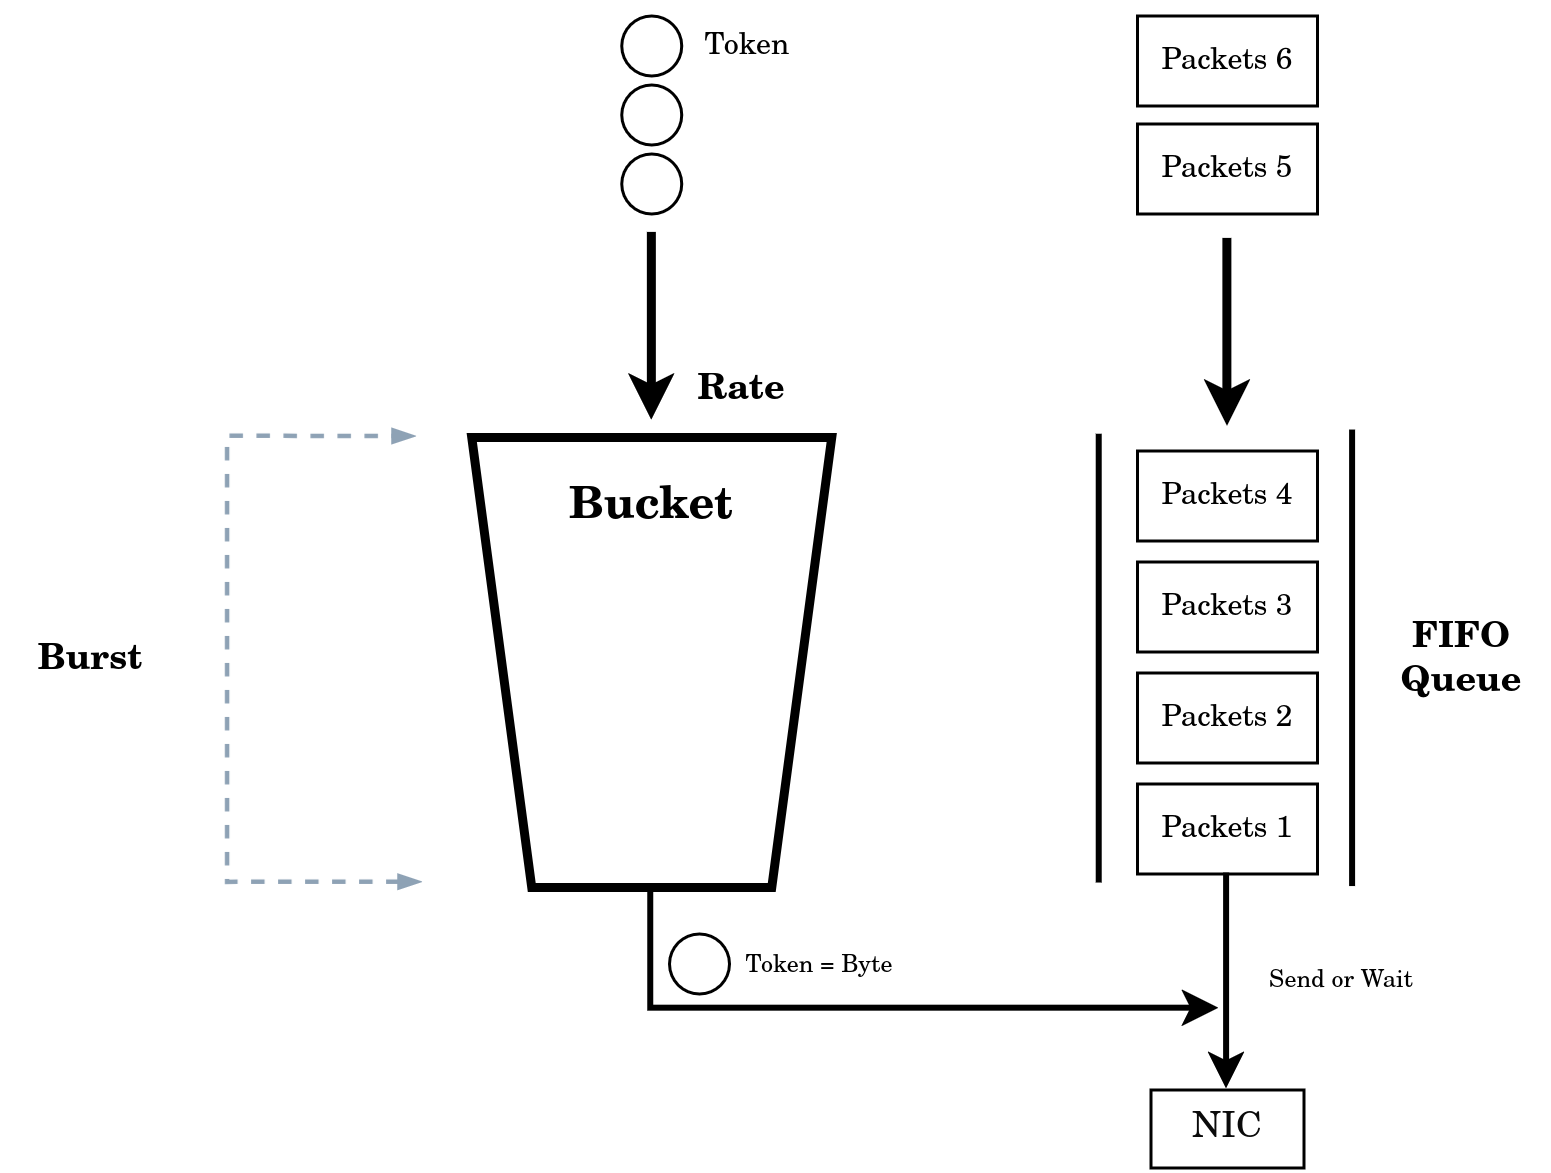
\includegraphics[width=0.7\linewidth]{Images/shaping/tbf.png}
    \caption{Funzionamento di TBF}
\end{figure}

La coda dei pacchetti utilizza una politica \textbf{FIFO} (First In, First Out) e la sua grandezza in byte può essere decisa tramite il parametro \textbf{limit}.
Se piena, i pacchetti successivi vengono scartati direttamente.
\vspace*{0.01\textheight}
\begin{center}
  \begin{tabular}{ |c|c|c| }
    \hline
    \multicolumn{3}{|c|}{\textbf{Parametri comando tc per TBF \cite{tc-tbf}}} \\
    \hline
    \textbf{Parametro} & \textbf{Unità di Misura} & \textbf{Descrizione} \\
    \hline
    rate & $\text{Mbit}/s$ & Velocità di generazione dei tokens. \\
    \hline
    burst & Byte & Capienza del bucket. \\
    \hline
    limit & Byte & Capienza della coda. \\
    \hline
  \end{tabular}
\end{center}

\newpage

\subsection{Hierachical Token Bucket (HTB)}
\begin{defn}[Hierachical Token Bucket]
  Disciplina di accodamento \textbf{classful} disponibile per il controllo del traffico nel comando \texttt{tc}. \\
  Utilizzato per fare traffic shaping controllando la banda in uscita di un interfaccia,
  permettendo di dividere vari flussi tramite l'uso di un albero per creare una \textbf{gerarchia di classi}. 
  L'algoritmo utilizzato per l'elaborazione del traffico è token bucket filter \cite{tc-htb}.
\end{defn}

Ogni classe rappresenta un nodo di un \textbf{albero} e, ad eccezzione della \textbf{radice}, ha una classe \textbf{genitore}.
Questa struttura permette di suddividere ricorsivamente la banda assegnata a una classe tra le sue classi figlie,
ciascuna configurabile con i propri parametri: \textbf{rate} e \textbf{ceil}. \\

\begin{figure}[!htb]
    \centering
    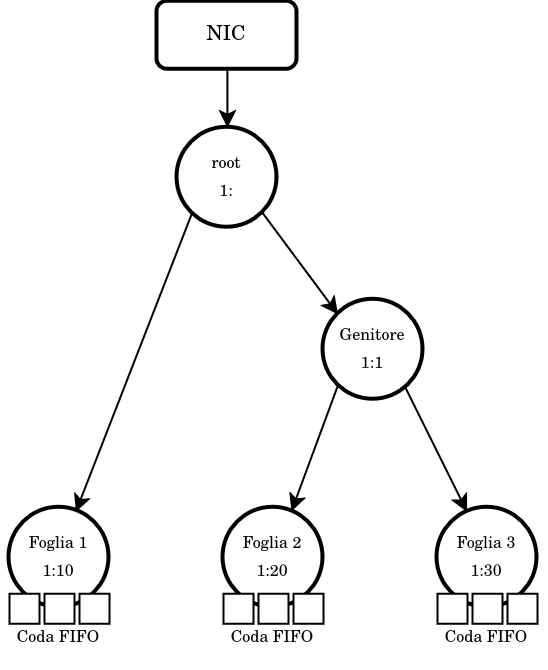
\includegraphics[width=0.5\linewidth]{Images/shaping/htb.png}
    \caption{Gerarchia HTB}
\end{figure}

Le code FIFO di pacchetti in attesa possono essere solo sulle foglie dell'albero, i nodi intermidi non possono accodare.

\subsubsection{Algortimo di Condivisione della Banda}
Tramite questo algoritmo, quando una classe necessita di più banda di quella garantita dal proprio rate,
può prendere in prestito la capacità non utilizzata dalle classi che condividono lo stesso genitore, fino al limite imposto dal proprio ceil.
Il parametro rate indica la banda \textbf{minima} garantita, invecem il parametro ceil indica la banda \textbf{massima} utilizzabile.\\
\vspace*{0.01\textheight}
Una classe genitore conosce la somma della banda effettivamente utilizzata dalle proprie classi figlie e può quindi ridistribuirla a quelle che ne richiedono di più.
Considerando che come algoritmo viene usato token bucket, possiamo includere tutti i casi possibili dei prestiti in tre situazioni diverse \cite{htb-site}:
\begin{itemize}
  \item Il numero di tokens di una classe è sufficiente per inviare immediatamente il pacchetto.
  \item Il numero di tokens di una classe non è sufficiente per inviare immediatamente un pacchetto, ma è possibile chiedere un prestito alla classe genitore, visto che la banda non è satura.
  \item Il numero di tokens di una classe non è sufficiente per inviare immediatamente un pacchetto e non è possibile prendere in prestito ulteriore banda. Il paccheto viene aggiunto alla coda finchè non sarà possibile spedirlo.
\end{itemize}
I parametri utli per l'algoritmo di prestito sono:
\vspace*{0.01\textheight}
\begin{center}
  \begin{tabular}{ |c|c|c| }
    \hline
    \textbf{Parametro} & \textbf{Unità di Misura} & \textbf{Descrizione} \\
    \hline
    rate & $\text{Mbit}/s$ & Velocità minima garantita di generazione dei tokens. \\
    \hline
    burst & Byte & Capienza del bucket. \\
    \hline
    ceil & Mbit$/s$ & Velocità massima possibile di generazione dei tokens. \\
    \hline
    cburst & Byte & Capienza del bucket necessaria quando la \\
     &  & generazione dei tokens è al massimo possibile.\\
    \hline
    quantum & Byte & Byte da inviare prima di passare a un'altra classe. \\
    \hline
  \end{tabular}
\end{center}

\subsubsection{Filtri}
\begin{defn}[Filtro]
  Metodo usato per inserire il pacchetto un una determinata classe in base a diverse caratteristiche, è possibile farli pure tramite il comando \texttt{tc} (traffic control) \cite{tc}.
  Non è l'unico modo pensato per classificare i pacchetti, possono essere usare pure le iptables \cite{iptables}.
\end{defn}
I filtri sono l'oggetto che lega le code code di pacchetti alle classi e possono farlo secondo vari criteri: ip, porte, protocolli, fwmark nel caso vengano usate le iptables e molti altri.

\begin{figure}[!htb]
    \centering
    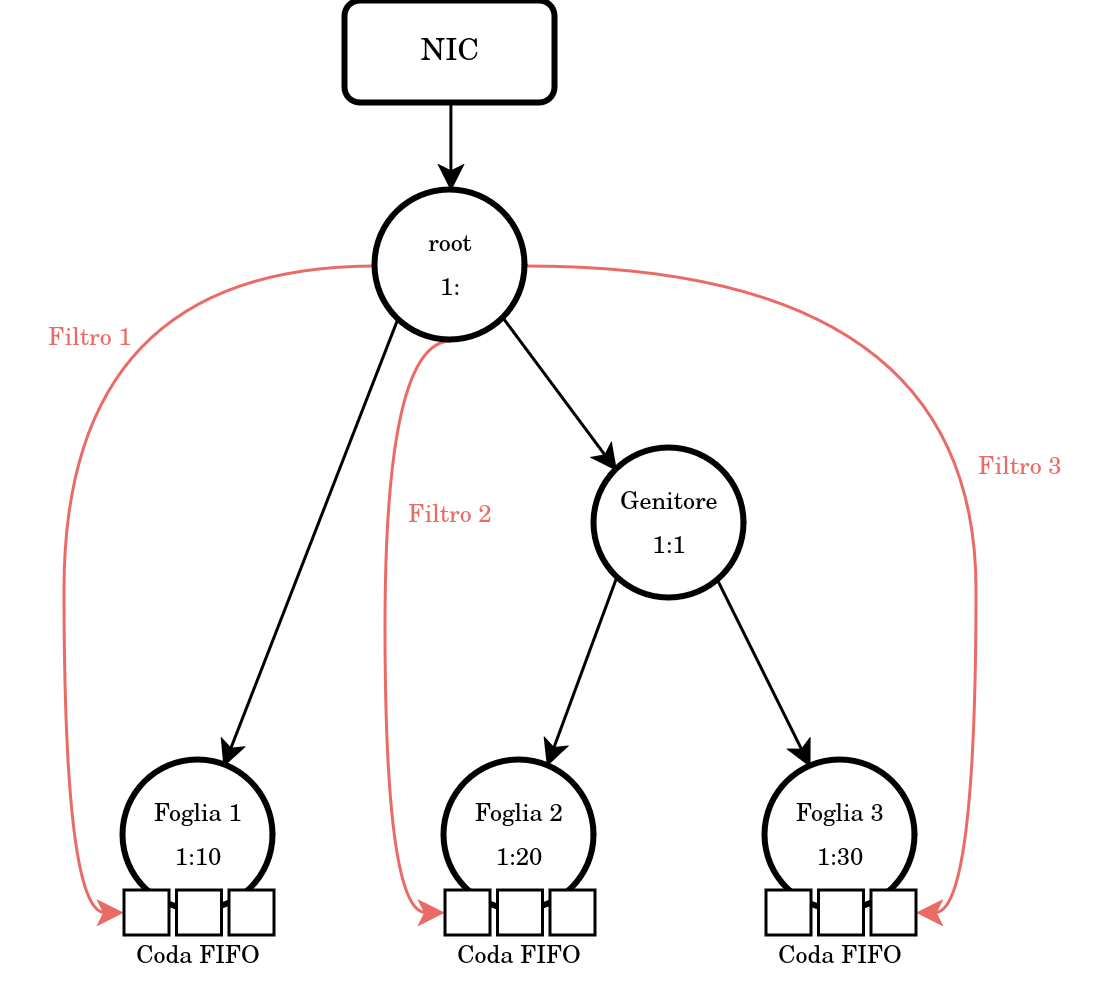
\includegraphics[width=0.6\linewidth]{Images/shaping/filtri.png}
    \caption{Classificazione pacchetti con filtri in HTB.}
\end{figure}
Normalmente la classificazione avviene una sola volta, con i filtri applicati al nodo radice, ma è possibile aggiungere ulteriori filtri nei nodi intermedi.

\newpage
\section{Esempi Reali di Utilizzo}
Il traffic shaping è usato anche i contesti reali. Nei prossimi paragrafi, vorrei mostrare alcuni casi d'uso in cui 
è utile applicare discipline di accodamento come Token Bucke Filter o Hierachical Token Bucket.

\subsection{Limitazione Banda su Backup}
\begin{note}[Scenario]
  Un piccolo ufficio ha una connessione internet condivisa da 20 Mbit/s in upload. Un server esegue un backup automatico verso il cloud in diversi orari della giornata
  e se lasciato libero satura completamente la banda in upload. Si vuole limitare la velocità del traffico il uscita in modo da permettere ai dipendenti di lavorare tranquillamente.
\end{note}

\begin{figure}[!htb]
    \centering
    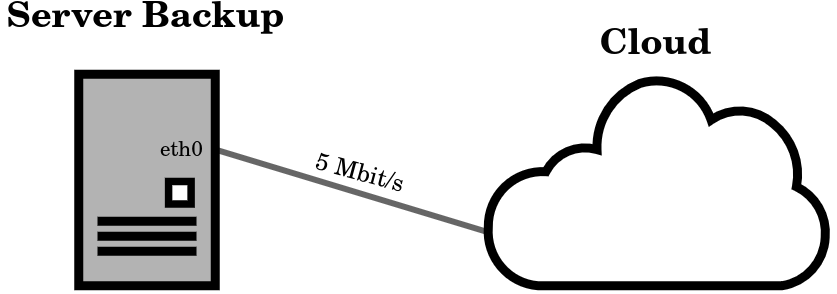
\includegraphics[width=0.6\linewidth]{Images/shaping/Es1.png}
    \caption{Rappresentazione grafica del primo scenario.}
\end{figure}

In questo caso, è possibili limitare il traffico sull'interfaccia di rete del server di backup. 
Ipotizziamo che l'interfaccia sia \texttt{eth0} e che si voglia limitare il traffico a $5$ Mbit$/s$:
\begin{bash}[Comando tc]
  tc qdisc add dev eth0 root tbf rate 5mbit burst 32kb limit 100kb
\end{bash}
Ora, la connessione è correttamente limitata. 

\subsection{Server con Multipli Servizi}
\label{sec:htb}
\begin{note}[Scenario]
  Un server di un'azienda ospita tre servizi per tre clienti diversi: un servizio streaming, un sito web con molto traffico e un servizio di file hosting. \\ 
  La banda totale disponibile e garantita è 100 Mbit/s. Si vuole garantire più banda al cliente del sito web rispetto agli altri due clienti.
  Gli altri due servizi avranno un minimo di banda garantita.
\end{note}

\begin{figure}[!htb]
    \centering
    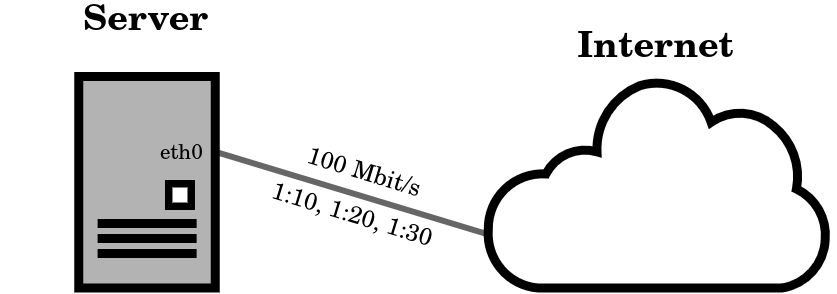
\includegraphics[width=0.6\linewidth]{Images/shaping/Es2.png}
    \caption{Rappresentazione grafica del secondo scenario.}
\end{figure}

In questo caso, con opportuni filtri è possibile inserire i pacchetti nelle code delle classi corrette: \texttt{1:10} per il sito web, \texttt{1:20} per lo streaming e \texttt{1:30} per il file hosting.
\begin{bash}[Classi e parametri con comando tc]
  # Nodo root e genitore
  tc qdisc add dev eth0 root handle 1: htb default 30
  tc class add dev eth0 parent 1: classid 1:1 htb rate 100mbit ceil 100mbit

  # Classe sito web
  tc class add dev eth0 parent 1:1 classid 1:10 htb rate 50mbit ceil 100mbit

  # Classe servizio streaming
  tc class add dev eth0 parent 1:1 classid 1:20 htb rate 35mbit ceil 60mbit

  # Classe servizio file hosting
  tc class add dev eth0 parent 1:1 classid 1:30 htb rate 15mbit ceil 20mbit
\end{bash}
Il nodo genitore ha un minimo e un massimo di banda di 100Mbit/s, che dividerà fra le tre classi, permettendo pure il prestito nel caso fosse possibile. \\
L'ultima cosa che rimane da fare è scrivere i vari filtri che divideranno il traffico nelle opportune code.

\begin{bash}[Filtri con comando tc]
  # Filtri per sito web
  tc filter add dev eth0 protocol ip parent 1:0 prio 1 u32 match ip sport 80 0xffff flowid 1:10
  tc filter add dev eth0 protocol ip parent 1:0 prio 1 u32 match ip sport 443 0xffff flowid 1:10

  # Filtro per servizio streaming 
  tc filter add dev eth0 protocol ip parent 1:0 prio 2 u32 match ip sport <port> 0xffff flowid 1:20

  # Filtro per servizio file hosting
  tc filter add dev eth0 protocol ip parent 1:0 prio 3 u32 match ip sport <port> 0xffff flowid 1:30
\end{bash}
In questo modo, il traffico in uscita con porta sorgente \texttt{80} e porta \texttt{443} (http e https), andrà correttamente nella classe creata per il sito web. 
I pacchetti degli altri due servizi verranno classficati, come fatto in precendenza, in base alla loro porta sorgente. \\ 
Nel comando è stata inserita un diversa priorità per la valutazione dei filtri.


\chapter{Kathará}
\section{Introduzione}
\begin{defn}[Kathará]
  Kathará è un framework open source basato su container Docker che permette di creare, configurare ed eseguire reti virtuali,
  integrando in un unico ambiente tecnologie come \textbf{SDN} (Software Defined Network) e \textbf{NFV} (Network Function Virtualization) \cite{8406267}.
\end{defn}
Ogni nodo di rete è simulato con un container. Il comportamento del nodo dipende dall'immagine usata,
permettendo l'uso di protocolli tradizionali (OSPF, BGP, ecc), SDN o servizi applicativi (DNS, Apache, ecc).
I vari dispositivi comunicano tra loro attraverso LAN virtuali di livello 2, riproducendo il comportamente di un collegamento fisico.\\
\vspace*{0.01\textheight}
La scelta di basarsi su container invece che su macchine virtuali, rende Kathará uno strumento molto leggero.
Ogni container richiede risorse nettamente inferiori rispetto a una macchina virtuale tradizionale, permettendo di simulare topologie complesse su hardware meno performante.
Inoltre, permette di sfruttare bene tecnologie come NFV (Network Function Virtualization), che utilizza funzioni software per sositutire dispositivi hardware,
e SDN (Software Defined Network), che permette di separare la logica di controllo della rete, dalla logica di invio dei pacchetti.

\section{Architettura di Kathará}
L'architettura di Kathará è composta da tre moduli principali: \textbf{Scripts}, \textbf{Operations} e il \textbf{Container Platform Adapter} \cite{8406267}.
\begin{figure}[!htb]
    \centering
    \includegraphics[width=0.65\linewidth]{Images/kathara/Kathara.png}
    \caption{Architettura di Kathará \cite{8406267}}
\end{figure}
\newpage
Il modulo Scripts contiene le operazioni di base che utente può fare per avviare, fermare e mettere in pausa i nodi di rete. Si dividono in due tipologie:
\begin{enumerate}
  \item \textbf{ltools:} valgono per tutti i nodi inseriti nel file di configurazione (\texttt{lstart}, \texttt{lclean}).
  \item \textbf{vtools:} valgono per un singolo nodo (\texttt{vstart}, \texttt{vclean}).
\end{enumerate}
Il modulo Operations, invece, racchiude alcune funzionalità che servono a Kathará per funzionare, come:
\begin{itemize}
  \item \textbf{Parser:} traduce i file di configurazione o i parametri passati da riga di comando in nodi della rete con eventuali collegamenti. 
    Si occupa anche di tradurre ulteriori opzioni, come risorse assegnate a ogni nodo o immagini Docker da utilizzare.
  \item \textbf{Start-Up Operations:} serve a garantire compabilità fra i diversi sistemi.
  \item \textbf{Common Libraries:} genera una serie di operazioni indipendenti da eseguire.
\end{itemize}
Infine, il modulo del Container Platform Adapter converte i comandi generati in precedenza in direttive Docker (o altre piattoforme) per creare e collegare fra di loro i container.
L'output dell'adapter ritorna al modulo Scripts, che lo invia al Docker daemon. \\
\vspace*{0.01\textheight}
Nei sistemi Unix, per ragioni di sicurezza, i comandi devono prima essere approvati da un wrapper che scarta qualsiasi comando non ritenuto sicuro.

\section{Configurazione}
Supponiamo di avere un rete con tre nodi: due host e uno switch. Tramite Kathará è possibile crearli e avviarli tramite riga di comando, con i vtools, oppure, tramite file di configurazione, con gli ltools \cite{8406267}.
Questa seconda modilità è quella che userò per configurare la rete.\\
\vspace*{0.01\textheight}
Il primo file da creare è quello in cui vengono definiti i nodi e se necessario altre opzioni, come le immagini dei container Docker. 
\begin{kathara}[lab.conf]
  # Collegamento fra un host e porte dello swicth
  pc1[0]="A"
  sw1[0]="A"

  pc2[0]="B"
  sw1[1]="B"

  # Immagine per lo switch
  sw1[image]="kathara/quagga"
\end{kathara}
Successivamente, è possibile creare a avviare i container con il comando \texttt{kathara lstart}, partendo dalle immagini di default o da quelle specificate. 
Kathará, inoltre, aprirà per ogni nodo un terminale, in modo da poter fare modifiche o test. \\
\vspace*{0.01\textheight}
In alternativa, è possibile creare dei file di configurazione per ogni nodo, scrivendo al suo interno una lista di comandi da far fare in automatico all'accensione del container.
Per l'host \texttt{pc1}, nel suo file di configurazione si può assegnare un ip e accendere la rispettiva interfaccia.
\begin{kathara}[pc1.startup]
  # Assegnare un ip
  ip addr add 192.168.1.1/24 dev eth0

  # Accendere l'interfaccia eth0
  ip link set dev eth0 up
\end{kathara}
Tramite questa modalità è possibile configurare pure il secondo host e lo swicth. Una volta digitato il comando \texttt{kathara lstart}, tutti i file di configurazione verrano usati per creare la rete.

\subsection{Riproduzione dello scenario HTB in Kathará}
Sfruttando Kathará, si possono riproporre gli esempi del capitolo precedente sull'utlizzo delle qdisc tramite il comando \texttt{tc}, testandolo con diversi nodi.
In particolare, lo scenario su HTB è utile per dimostrare che è possibile fare traffic shaping con questo framework.
\vspace*{0.01\textheight}
Facendo riferimento allo scenario dell'esercizio \ref{sec:htb}, il primo file da creare sarà \texttt{lab.conf}, in cui dovranno essere definiti i tre clienti e il server con i servizi.
\begin{kathara}[lab.conf]
  # Clienti
  c1[0] = "A"
  c2[0] = "A"
  c3[0] = "A"
  
  # Server
  server[0] = "A"
\end{kathara}
Specificando per ognuno il dominio \texttt{"A"}, Kathará simulerà il comportamente di una rete locale con uno swicth che collega tutti i nodi.
Successivamente, per ogni host, dovrà essere creato un file che conterrà tutti i comandi necessari per poter comunicare fra di loro e nel caso del server pure quelli utili per il traffci shaping.
\begin{kathara}[c1.startup]
  # Assegnazione ip
  ip addr add 10.0.0.1/24 dev eth0

  # Accensione interfaccia eth0
  ip link set dev eth0 up
\end{kathara}
Questa configurazione sarà uguale anche per gli altri clienti, ad eccezzione dell'indirizzo ip differente. Invece, in \texttt{server.startup}, verranno inseriti pure i comandi con \texttt{tc}.
\begin{bash}[server.startup]
  # Assegnazione ip
  ip addr add 10.0.0.10/24 dev eth0

  # Accensione interfaccia eth0
  ip link set dev eth0 up

  # Nodo root e genitore
  tc qdisc add dev eth0 root handle 1: htb default 30
  tc class add dev eth0 parent 1: classid 1:1 htb rate 100mbit ceil 100mbit

  # Classe sito web
  tc class add dev eth0 parent 1:1 classid 1:10 htb rate 50mbit ceil 100mbit

  # Classe servizio streaming
  tc class add dev eth0 parent 1:1 classid 1:20 htb rate 35mbit ceil 60mbit

  # Classe servizio file hosting
  tc class add dev eth0 parent 1:1 classid 1:30 htb rate 15mbit ceil 20mbit
\end{bash}
Infine, all'interno di quest'ultimo file, o sul container una volta avviato, dovranno essere creati pure i filtri per classificare i flussi.
\begin{bash}[server.startup]
  # Filtri per sito web
  tc filter add dev eth0 protocol ip parent 1:0 prio 1 u32 match ip sport 80 0xffff flowid 1:10
  tc filter add dev eth0 protocol ip parent 1:0 prio 1 u32 match ip sport 443 0xffff flowid 1:10

  # Filtro per servizio streaming
  tc filter add dev eth0 protocol ip parent 1:0 prio 2 u32 match ip sport 554 0xffff flowid 1:20

  # Filtro per servizio file hosting
  tc filter add dev eth0 protocol ip parent 1:0 prio 3 u32 match ip sport 21 0xffff flowid 1:30
\end{bash}

\subsubsection{Risultati}
Per capire gli effetti che il traffic shaping ha portato alla rete, è utile confrontare i tempi di invio di dati con o senza HTB. La formula per calcolare i tempi di invio ideali è:
\[
  t = \frac{\text{dim} \times 8}{\text{rate}}
\]
Sul nodo del server è stato creato un file di 100 MB e poi è stato posto in ascolto sulle tre porte: \texttt{443}, \texttt{554} e \texttt{21}. 
Ogni client ha scaricato contemporaneamente il file, tramite il comando \texttt{nc}, collegandosi alla porta del proprio servizio. \\ 
Per ciascun trasferimento è stato misurato il tempo reale.
\begin{center}
  \begin{tabular}{ |c|c|c| }
    \hline
    \textbf{Classe} & \textbf{Tempo Ideale} & \textbf{Tempo Reale} \\
    \hline
    1:10 & $\sim$ $16s$ & $19.20s$ \\
    \hline
    1:20 & $\sim$ $23s$ & $23.33s$ \\
    \hline
    1:30 & $\sim$ $53s$ & $48.47s$ \\
    \hline
  \end{tabular}
\end{center}
Nell'esempio, si può notare come la classe \texttt{1:30} abbia impiegato meno tempo di quello ideale. Questo è dovuto al fatto che,
dopo che il primo cliente ha finito di leggere i \texttt{100MB} di file, le altre due classi si sono divise la banda tramite l'algoritmo di prestito. \\
Inoltre, per capire l'effetto del traffic shaping nella rete, è utile guardare anche i risultati senza l'utilizzo di HTB.
\begin{center}
  \begin{tabular}{ |c|c|c| }
    \hline
    \textbf{Classe} & \textbf{Tempo} \\
    \hline
    Sito Web & $22.81s$ \\
    \hline
    Streaming & $23.04s$ \\
    \hline
    File Hosting & $24.64s$ \\
    \hline
  \end{tabular}
\end{center}
Si può notare come i tempi, simili tra loro, rappresentino un terzo della banda totale, ossia circa 33Mbit/s per ciascun nodo, 
dato che $\frac{100 \text{MB} \times 8}{33 \text{Mbit}/s} = 24s$. \\
\vspace*{0.01\textheight}
In conclusione, applicando una disciplina di accodamento come HTB per fare traffic shaping,
ha permesso al servizio del sito web di avere a disposizione una banda maggiore, terminando il trasferimento per primo. 
Invece, ha rallentato il servizio di file hosting, dedicandogli una banda minore. \\
L'utilizzo di Kathará per creare la rete, ha permesso di calcolare i tempi reali in una LAN nelle diverse modalità proposte.
\begin{center}
  \begin{tabular}{ |c|c|c|c| }
    \hline
    \textbf{Servizio} & \textbf{Tempo con HTB} & \textbf{Tempo senza HTB}\\
    \hline
    Sito Web & $19.20s$ & $22.81s$ \\
    \hline
    Streaming & $23.33s$ & $23.04s$ \\
    \hline
    File Hosting & $48.47s$ & $24.64s$ \\
    \hline
  \end{tabular}
\end{center}

\newpage
\section{Dipendenza dai moduli del kernel host}
L'uso di container Docker rende la simulazione leggera e flessibile, permettendo di scegliere per ogni nodo un'immagine diversa, ma crea un limite imporntante.
A differenza delle macchine virtuali, i container non eseguono un kernel proprio, ma condividono quello dell'host su cui gira Docker, 
ciò che un nodo può fare a livello di rete dipende dai moduli caricati nel kernel dell'host. \\
\vspace*{0.01\textheight}
Il comando tc, eseguito dentro un container, iniva solamente richieste al kernel, non implementa effettivamente le discipline di accodamento.
Le qdisc, le classi e i filtri sono realizzati da diversi moduli del kernel:
\begin{center}
  \begin{tabular}{ |c|c| }
    \hline
    \textbf{Modulo} & \textbf{Descrizione} \\
    \hline
    \texttt{sch\_tbf} & Modulo per qdisc TBF \\
    \hline
    \texttt{sch\_htb} & Modulo per qdisc HTB \\
    \hline
    \texttt{cls\_u32} & Modulo per filtri \texttt{u32} \\
    \hline
  \end{tabular}
\end{center}





\printbibliography[title={Bibliografia}] 

\end{document}
